\subsection{Bayesian Optimization}
\label{sec:bo}

Bayesian optimization approximate black-box functions with proxy functions and
iteratively proposes new sample point in the large parameter space. Effective
for,

\begin{itemize}
\item Evaluating each sample is expensive.
\item The objective is a black-box.
\item The evaluation can be noisy
\end{itemize}

Gaining attraction beyond ML scope:
\begin{itemize}
\item CherryPick~\cite{alipourfard2017cherrypick} finds the best cloud
  configurations for big data analytics.
\item Google optimize chocolate chip cookies recipes~\cite{solnik2017bayesian}.
\end{itemize}

\begin{figure}
  \centering
  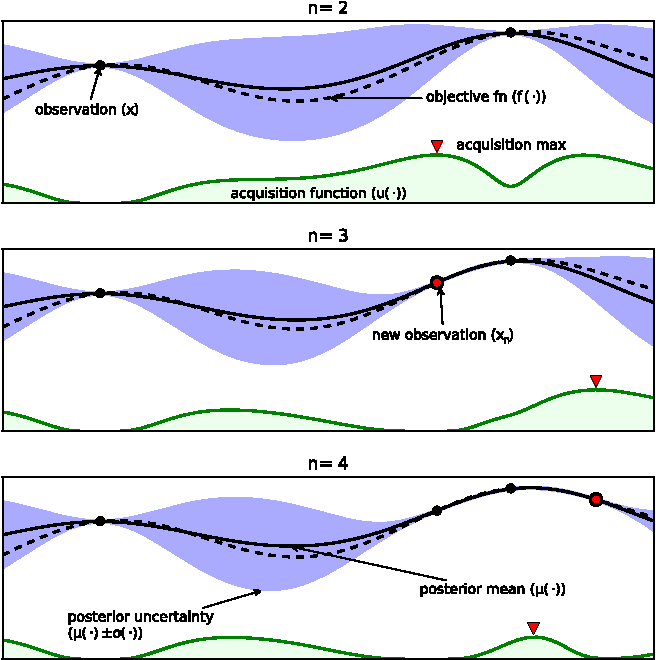
\includegraphics[width=0.8\textwidth]{figures/serving-bo-illustration.pdf}
  \caption{Acquisition function evaluates the utility of candidate points for
    the next evaluation of $f$, balancing a high objective (exploitation) and
    high uncertainty (exploration)~\cite{shahriari2016taking}}
\end{figure}

\begin{figure}
  \centering
  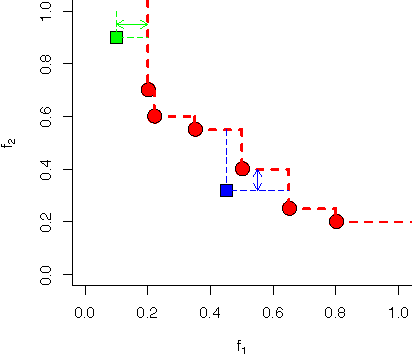
\includegraphics[width=0.8\textwidth]{figures/serving-bo-2d-1.pdf} \\
  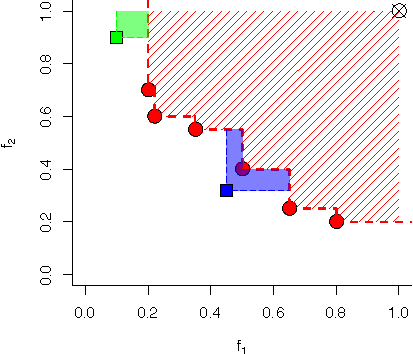
\includegraphics[width=0.8\textwidth]{figures/serving-bo-2d-2.pdf}
  \caption{For two-objective optimization, utility gain is based on
    additive-epsilon (top) or hypervolume (bottom)~\cite{binoisgpareto}}
\end{figure}

We use PESMO~\cite{hernandez2016predictive} and compare it with two baselines:
(1) greedy/coordinate search; (2) random search. PESMO chooses evaluation points
to maximally reduce the entropy of the posterior distribution over the Pareto
set.

%%% Local Variables:
%%% mode: latex
%%% TeX-master: "../compute"
%%% End:
